\chapter{Lowest Common Ancestor}
\section{Introduction}
The Lowest Common Ancestor (LCA) of two nodes $v$ and $w$ in a tree or directed acyclic graph (DAG) $T$ is the lowest (i.e. deepest) node that includes both v and w as descendants, where each node is defined as a descendent of itself in graph theory and computer science (so if $v$ has a direct connection from $w$, $w$ is the lowest common ancestor).In the development of object-oriented programming systems, the challenge of determining lowest common ancestors of classes in an inheritance hierarchy arises.The LCA problem also has applications in distributed computing models of complex systems.

\section{$k^{th}$ ancestor}
We need to solve the following problem: Given a tree with $N$ nodes, answer $Q$ queries. The $i^{th}$ query will contain two integers $a_i,b_i$ where $a_i$ is a node of the tree. The answer to the $i^{th}$ query is a node $p$ , such that $p$ is the $b_i^{th}$ ancestor of node $a_i$.\\
The naive approach to solve this problem would be to store the parent of each node in an array, and to run a simple for loop to find the $k^{th}$ ancestor. The worst case time complexity of this approach would be $O(N)$ for each query, and hence the overall complexity will be $O(NQ)$. Now, ofcourse it's time to ask the most clichéd question - Can we do better?\\
Let's try to come up with some possible approach to solve this.\\
\clearpage
\subsection{Idea for Binary Lifting}
Let's assume that for every node $x$, we know all the ancestors of $x$ that are perfect powers of two. That means, we know the $1^{st} , 2^{nd}, 4^{th} , 8^{th} \cdots$ ancestors of node $x$.Can we somehow use this data to find any ancestor of node $x$? Well, let's see: \\
Let's say we want to find the $6^{th}$ ancestor of node $x$. Let's say, $y$ is the $4^{th}$ ancestor of node $x$. Realize that,\\
\begin{figure}[h]
    \centering
    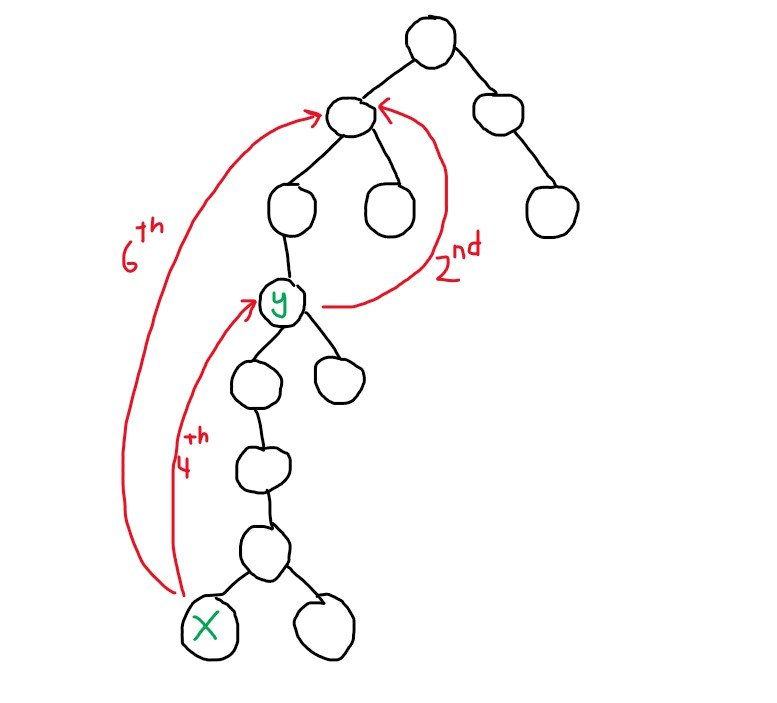
\includegraphics[scale=0.5]{images/lifting.jpg}
    \caption{Binary Lifting}
    \label{fig:my_label}
    
\end{figure}
\\ $$6^{th} \text{ancestor of node x} = 2^{nd} \text{ancestor of node y}$$

You might have already realized what to do by now. Let $b[i]$ represent the $i^{th}$ bit of number x. If the $i^{th}$ bit is set, i.e. $b[i] = 1$, then find the $2^{i}$th ancestor of node $x$, and reset the value of $x$ such that $x = 2^{i}\text{th ancestor of x}$. \\
For example, the bitwise representation of $14$ is $1110$. So, find the $8^{th}$ ancestor of $4^{th}$ ancestor of $2^{nd}$ ancestor of node $x$, and that shall be our final answer.\\
For some reason, I always refer to this method as "Anti Divide and Conquer" (unofficial). This is because - unlike divide and conquer, where we divide the problem into powers of two - we build up the powers of two solve this problem. Anyways, we considered the powers of two ancestors as black box. Now, we shall look at how to build these powers of two.

\subsection{Algorithm for Binary Lifting}
Let's see how to find the powers of two ancestors first:\\

\begin{minted}
[
frame=lines,
framesep=2mm,
baselinestretch=1.2,
fontsize=\footnotesize,
linenos
]
{cpp}
void dfs(int ver)
{
    vis[ver] = true;
    for(int i=1; i<30; i++)
    {
        if(ancestor[ver][i-1] != -1)
            ancestor[ver][i] = ancestor[ancestor[ver][i-1]][i-1];
        else
            ancestor[ver][i] = -1;
    }
    for(auto &i : v[ver])
    {
        if(vis[i] == false)
        {
            ancestor[i][0] = ver;
            depth[i] = depth[ver] + 1;
            dfs(i);
        }
    }
}
\end{minted}
This is an application of dynamic programming which works as follows: $\text{ancestor}[i][j]$ is the $2^j{th}$ ancestor of node $i$.We set $\text{ancestor}[\text{root}][0] = -1$. When we iterate through the children of node $i$, we set $\text{ancestor}[\text{child of } i][0] = i$. \\
Then we use the following rule to find the $2^{j}$th ancestor:\\
\begin{equation*}
    \text{ancestor}[i][j]=
    \begin{cases}
      \text{ancestor}[\text{ancestor}[i][j-1]][j-1], & \text{if}\ \text{ancestor}[i][j-1] != -1 \\
      -1, & ,\text{otherwise}
    \end{cases}
\end{equation*}
While doing so, also compute the depth of each node. The reason shall be explained later. \clearpage

Now we see how to compute the $k^{th}$ ancestor.\\
\begin{minted}
[
frame=lines,
framesep=2mm,
baselinestretch=1.2,
fontsize=\footnotesize,
linenos
]
{cpp}
int kthancestor(int v, int k)
{
    int node = v;
    for(int i=0; i<30; i++)
    {
        if(k & (1 << i))
            node = ancestor[node][i];
    }
    return node;
}
\end{minted}

As discussed earlier, we find the bitwise representation of $k$.  Let $b[i]$ represent the $i^{th}$ bit of number $k$. If the $i^{th}$ bit is set, i.e. $b[i] = 1$, then find the $2^{i}$th ancestor of node $x$, and reset the value of $k$ such that $k = 2^{i}\text{th ancestor of x}$.

\subsection{Complexity Analysis}
Excluding precomputation time for powers of two (which takes $O(N \logN)$), each query takes $O(\log N)$ time. So, the overall time complexity is $O(Q \log N)$. Space complexity would be $O(N \log N)$ for the ancestor array.
\clearpage
\section{Lowest Common Ancestor(LCA)}
Problem Statement: Given two nodes $u$ and $v$ of a tree, find a node $w$, such that $w$ is the node with highest depth, having both $u$ and $v$ as it's descendants.\\
Now that we know how to find the $k^{th}$ ancestor of a node, this is rather simple.Remember, we included a depth[ ] array earlier in the dfs() code? This is where we will use it. The first obvious step would be to bring $u$ and $v$ to the same level. Without any loss of generality, $\text{depth}[u] \ge \text{depth}[v]$.\\
So, the difference in their levels would be $x = \text{depth}[u] - \text{depth}[v]$. 
\begin{figure}[h]
    \centering
    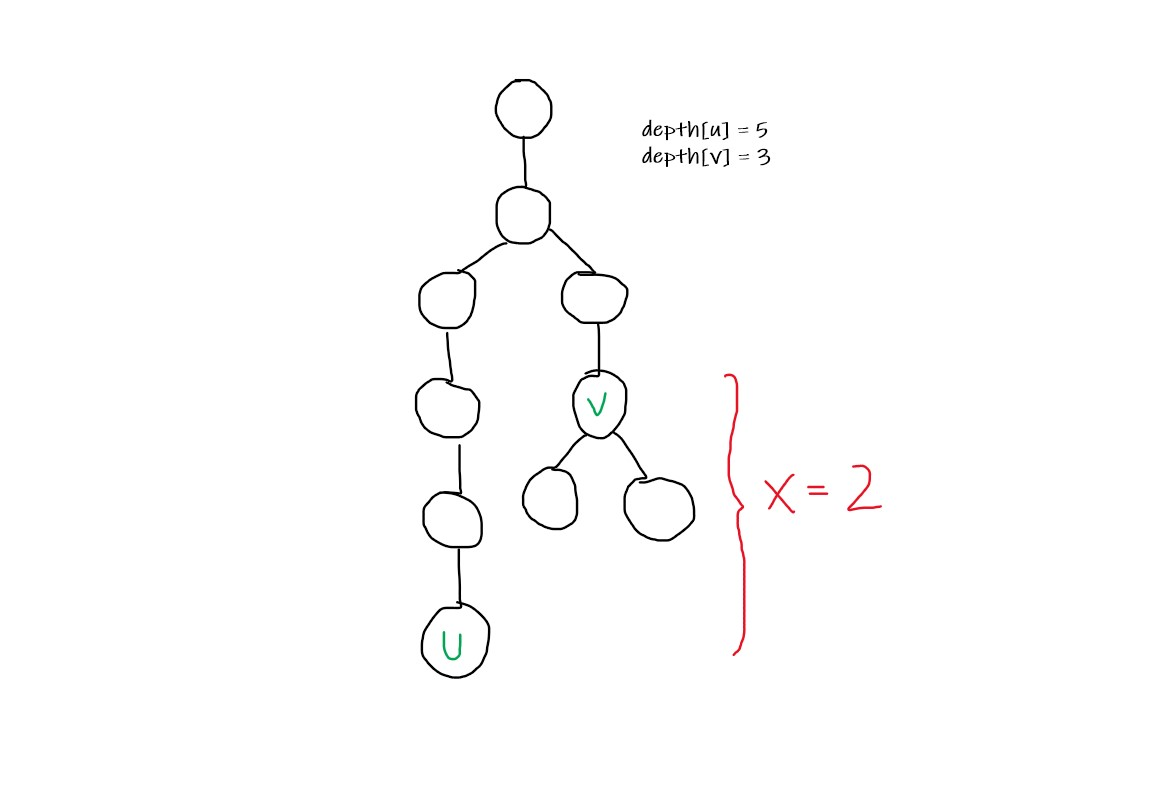
\includegraphics[scale=0.6]{images/lca.jpg}
    \caption{LCA}
    \label{fig:my_label}
\end{figure}
Now that $u$ and $v$ are at the same level, let's say $k^{th}$ ancestor of $u$ (and $v$) is the LCA. Then, $\forall p \in [k,\infty)$ , the $p^{th}$ node is also a common ancestor. So, starting from the MSB, we find the highest bit such that the ancestors of $u$ and $v$ are not common, and move it upto that level accordingly. 
The code would look as follows:
\begin{minted}
[
frame=lines,
framesep=2mm,
baselinestretch=1.2,
fontsize=\footnotesize,
linenos
]
{cpp}
int LCA(int a, int b)
{
    if(depth[a] < depth[b])
        swap(a,b);
    a = kthancestor(a , depth[a] - depth[b]);
    if(a == b)
        return a;
    for(int i=30; i>=0; i--)
    {
        if(ancestor[a][i] != ancestor[b][i])
        {
            a = ancestor[a][i];
            b = ancestor[b][i];
        }
    }
    return ancestor[a][0];    
}
\end{minted}
\subsection{Complexity Analysis}
The time and space complexity would be the same as binary lifting, i.e. $O(N \log N$) each.
